%-----------------------------------------------------------------------------%
\chapter{\babTiga}
%-----------------------------------------------------------------------------%

Penelitian ini dibagi menjadi empat tahap: (1) Mendapatkan data microarray dan pengolahan awal; (2) Perancangan algoritma; (3) Melakukan eksperimen untuk mendapatkan hyper parameter yang optimal. Kemudian dilanjutkan dengan  testing dan evaluasi. Gambaran umum dari penelitian ini seperti pada gambar bagan 1

\todo { untuk sementara copy paste dari laporan}

%-----------------------------------------------------------------------------%
\section{Gambaran Umum Penelitian}
%-----------------------------------------------------------------------------%

\todo { include grafik \\
\\
 }
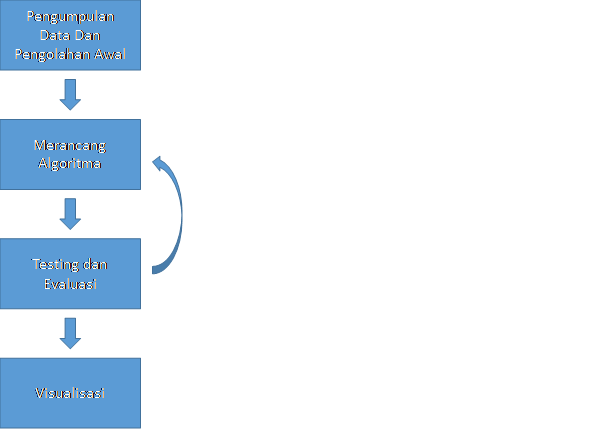
\includegraphics[scale=1]{pics/gbr3_1.png} 


%-----------------------------------------------------------------------------%
\section{Pengumpulan Data dan Pengolahan Awal}
%-----------------------------------------------------------------------------%
Data microarray tersedia secara bebas di geo [http://www.ncbi.nlm.nih.gov/geo/], dan dapat diunduh, untuk digunakan sebagai data penelitian. Kemudian dilakukan normalisasi standar yang sering di pakai pada data microarray, proses normalisasi ada banyak metode, dan akan digunakan satu metode standar untuk pengolahan awal microarray agar mendapatkan data konsisten dan dapat dibandingkan. Proses pengolahan awal dan normalisasi digunakan tools standar dan tersedia bebas yaitu R-Bioconductor. \\



%-----------------------------------------------------------------------------%
\section{Perancangan Algoritma}
%-----------------------------------------------------------------------------%



%-----------------------------------------------------------------------------%
\section{Melakukan Testing Arsitektur Deep Learning}
%-----------------------------------------------------------------------------%


%-----------------------------------------------------------------------------%
\section{Implementasi Metode Perangkingan Bobot Secara Multi Step Untuk Mendapatkan Gen Biomarker}
%-----------------------------------------------------------------------------%



%-----------------------------------------------------------------------------%
\section{Evaluasi Hasil Perangkingan Dengan Klasifikasi Secara Unsupervised}
%-----------------------------------------------------------------------------%



%-----------------------------------------------------------------------------%
\section{Perbandingan Hasil Perangkingan Dengan Literatur}
%-----------------------------------------------------------------------------%



